%!TEX root = Tesi.tex

\section{Progettazione sniffer}
Il primo passo per lo sviluppo è stato prendere confidenza sia con l'ambiente di lavoro che con il dispositivo della RedBear. Testare un semplice progetto, come il lampeggio di un led, si è comunque rivelata un'operazione non banale.
L'SDK che la Nordic fornisce contiene esempi modificati appositamente per le sue board di sviluppo, come la PCA10040 o la PCA10056, descritte nel capitolo \ref{nordic_board}, che come già accennato hanno una piedinatura e una dotazione di periferiche differente rispetto al nano2. Il primo passo è stato quindi quello di utilizzare una board supportata e modificarne la piedinatura delle periferiche connesse; il numero di led è stato ridotto a 1 solo connesso al pin 11 e sono stati rimossi i riferimenti a pulsanti connessi, perché non presenti sulla nostra periferica. \'E stato necessario modificare anche i collegamenti dei 4 pin relativi alla comunicazione UART come segue:
\begin{itemize}
\item[-] CTS pin 28
\item[-] RTS pin 2
\item[-] TX pin 29
\item[-] RX pin 30
\end{itemize}
Tutte queste modifiche sono state apportate al file pca10040.h che si trova nell'sdk nella cartella /components/boards .

Eseguendo una nuova compilazione e provando a scrivere il file .hex generato continuava a non funzionare. Dopo varie prove si è capito che mancavano delle librerie da cui il progetto dipendeva; esse sono contenute nel SOFTDEVICE, un file .hex che viene fornito già compilato nell'SDK, nella cartella /components/softdevice/s132/hex. Per tutti i progetti creati si usa la versione s132 del softdevice che è la più completa e contiene tutte le librerie necessarie per far funzionare il nano2 sia come dispositivo di tipo central che peripheral.

\subsection{UART}
Per visualizzare i dati intercettati via etere è necessario poter comunicare informazioni ad un dispositivo dotato di output video; nel nostro caso è stato utilizzato un PC, che avendo una gran capacità di memorizzazione può contenere tutti i dati catturati, per essere visualizzati ed analizzati anche in un secondo momento. Per trasferire questi dati abbiamo utilizzato una funzionalità supportata dal nano2, la trasmissione usando UART. \'E l'acronimo di Universal Asynchronous Receiver Transmitter, ovvero ricevitore trasmettitore asincrono/seriale, è un dispositivo hardware che converte flussi da un formato parallelo, tipicamente quelli usati all'interno di un processore, in formato seriale asincrono.
Inviare dati tramire UART è un'operazione che richiede pochi settaggi e quindi poche righe di codice, utilizzando le apposite funzioni di libreria messe a disposizione nella SDK. 

\begin{samepage}
All'interno di un progetto, va prima inizializzato il modulo fornendo le impostazioni che desideriamo usare:
\begin{itemize}
\item[-] Baudrate: il numero di simboli che vengono trasmessi in un secondo, determina la velocità di trasmissione.
\item[-] Control Flow: indica se utilizzare o meno le due linee aggiuntive destinate alla comunicazione UART ovvero, CTS (Clear To Send) e RTS (Ready To Send) per gestire lo scambio di dati, utile per annullare i conflitti trasmissivi.
\end{itemize}
Normalmente i settaggi sono inseriti nella funzione \emph{uart\_init()} che viene eseguita all'avvio del dispositivo.
\end{samepage}

Vanno inseriti dei caratteri di controllo per differenziare la fine di un pacchetto con l'inizio del successivo, ed eventualmente indicare informazioni aggiuntive al solo pacchetto, come la lunghezza dello stesso. \'E quindi stato inserito il carattere denominato MARKER del valore di 0xE0 all'inizio di ogni dato inserito; i 2 Byte successivi indicano la lunghezza dell'intero pacchetto, quindi comprendono anche i caratteri di controllo. Il quarto Byte viene usato per indicare il canale il cui è stato catturato il pacchetto e dal 5° Byte in poi si avrà ciò che è stato catturato, così come viene rilevato dal Nano2.
\begin{figure}[H]
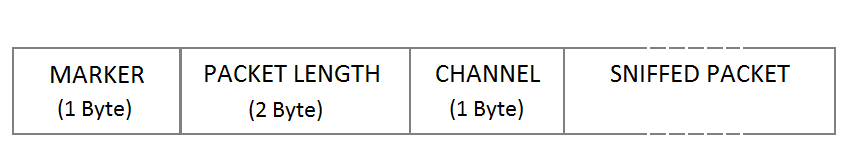
\includegraphics[width=300pt]{uart_packet}
\centering
\caption{Pacchetto inviato tramite UART che contiene il pacchetto sniffato e i campi di controllo.}
\end{figure}
Nel caso in cui all'interno del pacchetto stesso ci siano Byte del valore di 0xE0, che hanno lo stesso valore del Marker, per evitare di confonderli si raddoppia il Byte. In questo modo se nel pacchetto ricevuto si incontrerà un Byte singolo del valore del Marker, allora quello sarà un vero Marker che indica l'inizio di una nuova trasmissione; negli altri casi sarà un Byte del pacchetto, si dovrà quindi scartare il Byte successivo, che non fa parte dei dati catturati dallo Sniffer.

\subsection{NRF RADIO}

